
%-------------------------------------------------------------------------------------------
%%%%%%%% PREAMBLE
%-------------------------------------------------------------------------------------------
\documentclass[11pt]{article}

% Load packages
\usepackage[T1]{fontenc}

\usepackage{aeguill}
\usepackage{fancyhdr, amssymb, amsmath, geometry,setspace,lastpage,pdflscape}
\usepackage[pdftex]{graphicx,color}
\definecolor{dkblue}{rgb}{0,0.08,0.45}
\usepackage[pdftex]{hyperref}
\hypersetup{colorlinks}%
%citecolor=black,%
%filecolor=black,%
%linkcolor=black,%
%urlcolor=black}

%\usepackage{lmodern}
\usepackage{helvet}
\renewcommand{\familydefault}{\sfdefault}

% Page Setup
\geometry{ top = 1in, bottom = 1in , left=1in, right=1in}
\pagestyle{empty}
\lhead{}
\chead{}
\rhead{}
\lfoot{}
\cfoot{\footnotesize \thepage  { /}  \pageref{LastPage}}
\rfoot{}

% Paragraph Setup
\setlength{\parskip}{\baselineskip}%
\setlength{\parindent}{0pt}%

% Title Information
\title{}
\author{}
\date{}

%-------------------------------------------------------------------------------------------
%%%%%%%% DOCUMENT BEGINS HERE
%-------------------------------------------------------------------------------------------
\begin{document}

\begin{center}
{\Large Main Text Figures}
\end{center}
\vspace{50pt}




%-------------------------------------------------------------------------------------------
% Figure 1 - Garki results
%-------------------------------------------------------------------------------------------

\begin{figure}[htbp]
\begin{center}
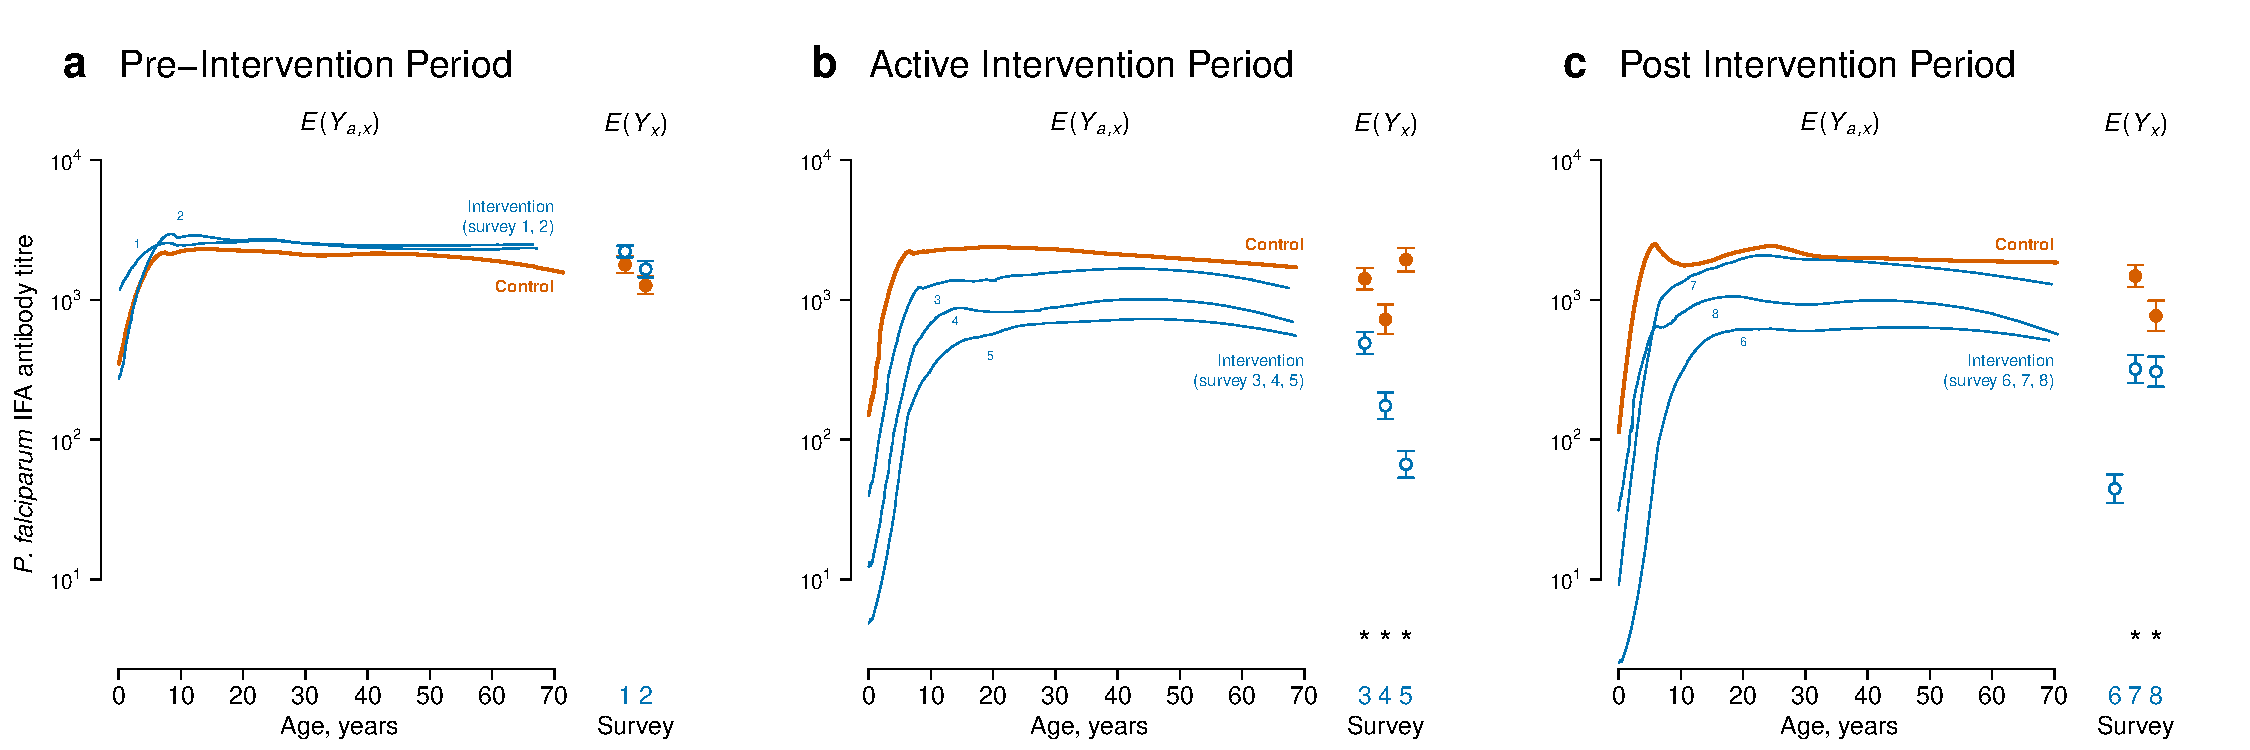
\includegraphics[width=\textwidth]{/users/benarnold/SLAbcurves/results/figs/garki-antibody-curves-IFAPf.pdf} \\ 
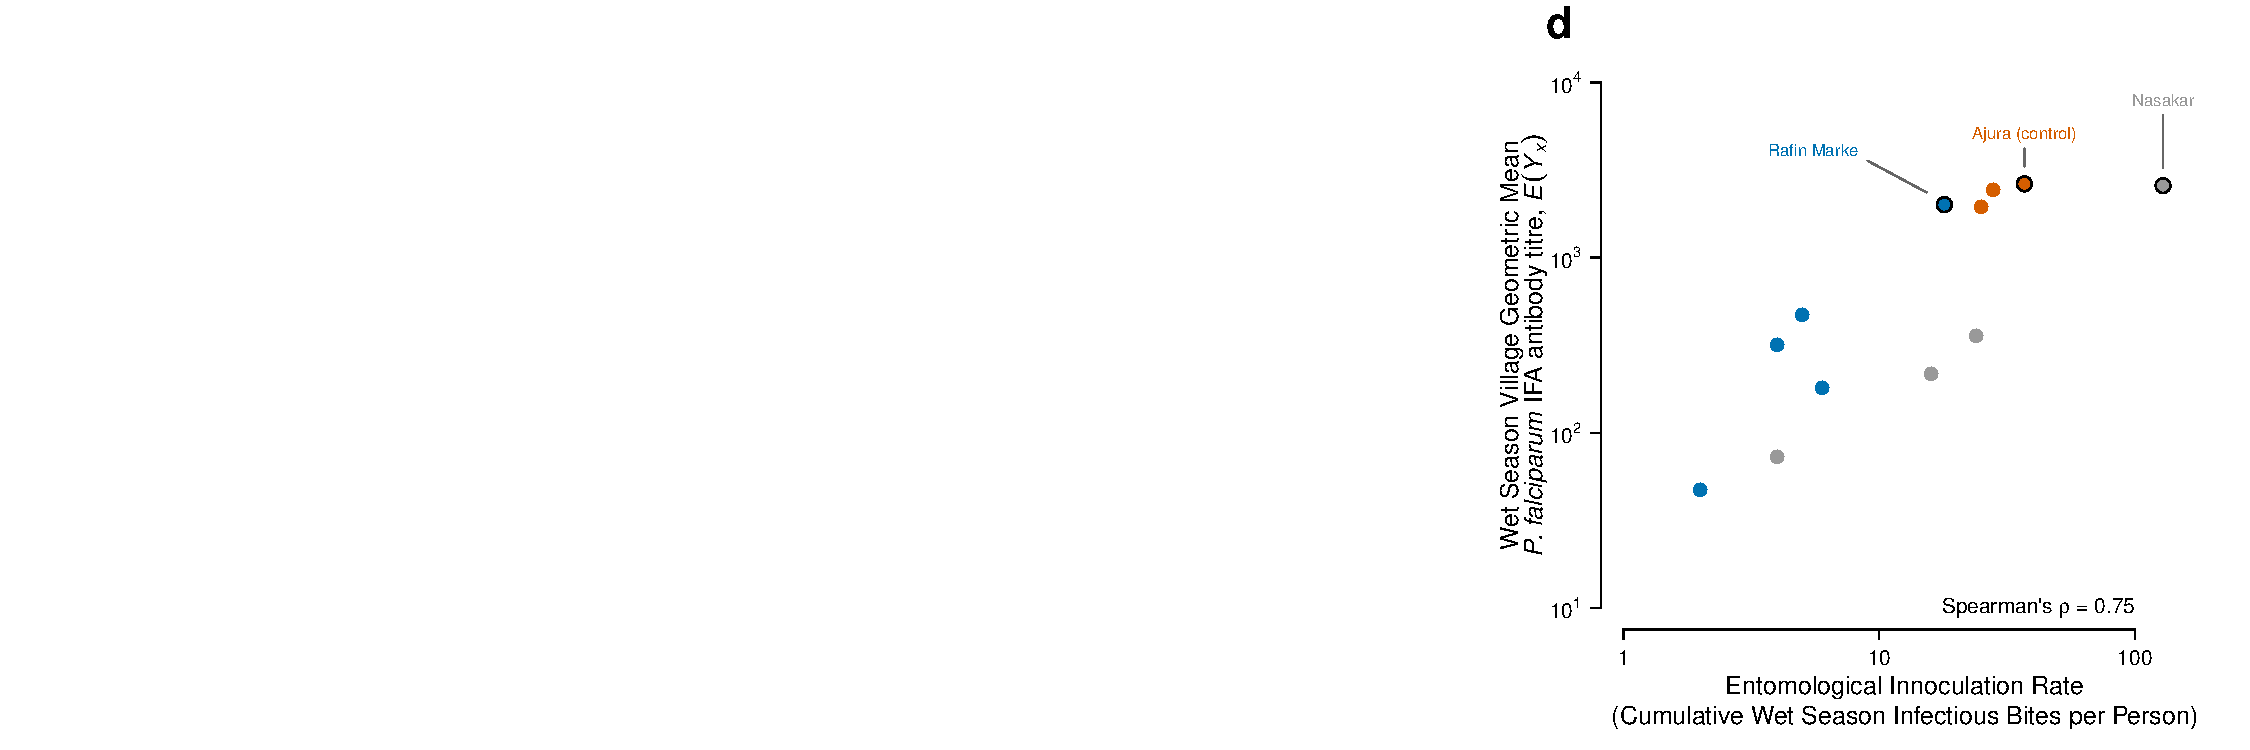
\includegraphics[width=\textwidth]{/users/benarnold/SLAbcurves/results/figs/garki-IFAPf-EIR.pdf}
\begin{minipage}{\textwidth}
\caption{Age-specific antibody response curves measure changes in malaria transmission due to intervention in the Garki Project, Nigeria (1970-1976). The intervention included a combination of insecticide spraying and mass drug administration of surfanene-pyrimethamine in 1972-1973, along with targeted distribution of chloroquine to children <10 and self-reporting fever cases in the 1974-75 post-intervention period. Antibody response measured with the indirect fluorescent antibody (IFA) test for \textit{Plasmodium falciparum}. \textbf{a}, pre-intervention period wet and dry seasons measures (survey rounds 1-2); \textbf{b}, active intervention period (survey rounds 3-5, at 20, 50, and 70 weeks following the start of intervention); \textbf{c}, post-intervention period (survey rounds 6-8 at 20, 40, and 90 weeks following the end of the intervention).  Age-specific antibody curves, $E(Y_{x,a})$ by group ($x$) and age ($a$), were estimated nonparametrically from quantitative antibody responses in individuals (N=6,024) using an ensemble machine learning algorithm (Online Methods). Control measurements were combined across survey rounds within each period when plotting the curves to facilitate visual comparison of shifts in transmission intensity between surveys. Age-adjusted geometric means by group, $E(Y_x)$, provide summary differences between curves at each survey round. Error bars show 95\% confidence intervals for the age-adjusted geometric means and asterisks indicate $P\leq0.01$ (Bonferroni corrected) for differences between control and intervention groups. Control villages were not measured in survey 6. \textbf{d}, Village-level, age-adjusted geometric mean \textit{P. falciparum} IFA titres, $E(Y_x)$, versus wet season entomological innoculation rate (EIR) in the three study villages with both entomological and serological measurements. Ajura was a control village (no treatment) while Rafine Marke and Nasakar were intervention villages.  The circled and labeled points are from the 1971 wet season (pre-intervention) and other points represent wet seasons for 1972-73 (Ajura) or 1972-75 (Rafine Marke and Nasakar). A single data point outside the figure range is not shown (Nasakar 1972, EIR value = 0, $E(Y_x) = 10^{3.0591}$), but was included in the Spearman rank correlation estimate.   }
\label{fig:garki}
\end{minipage}
\end{center}
\end{figure}

% note: timing of surveys estimated from Figs 1, 2 and 4 of Cornille-Broger 1978 Bull World Health Org  56 (4): 579-600


%-------------------------------------------------------------------------------------------
% Figure 2 - Mauke results
%-------------------------------------------------------------------------------------------
\begin{figure}[htbp]
\begin{center}
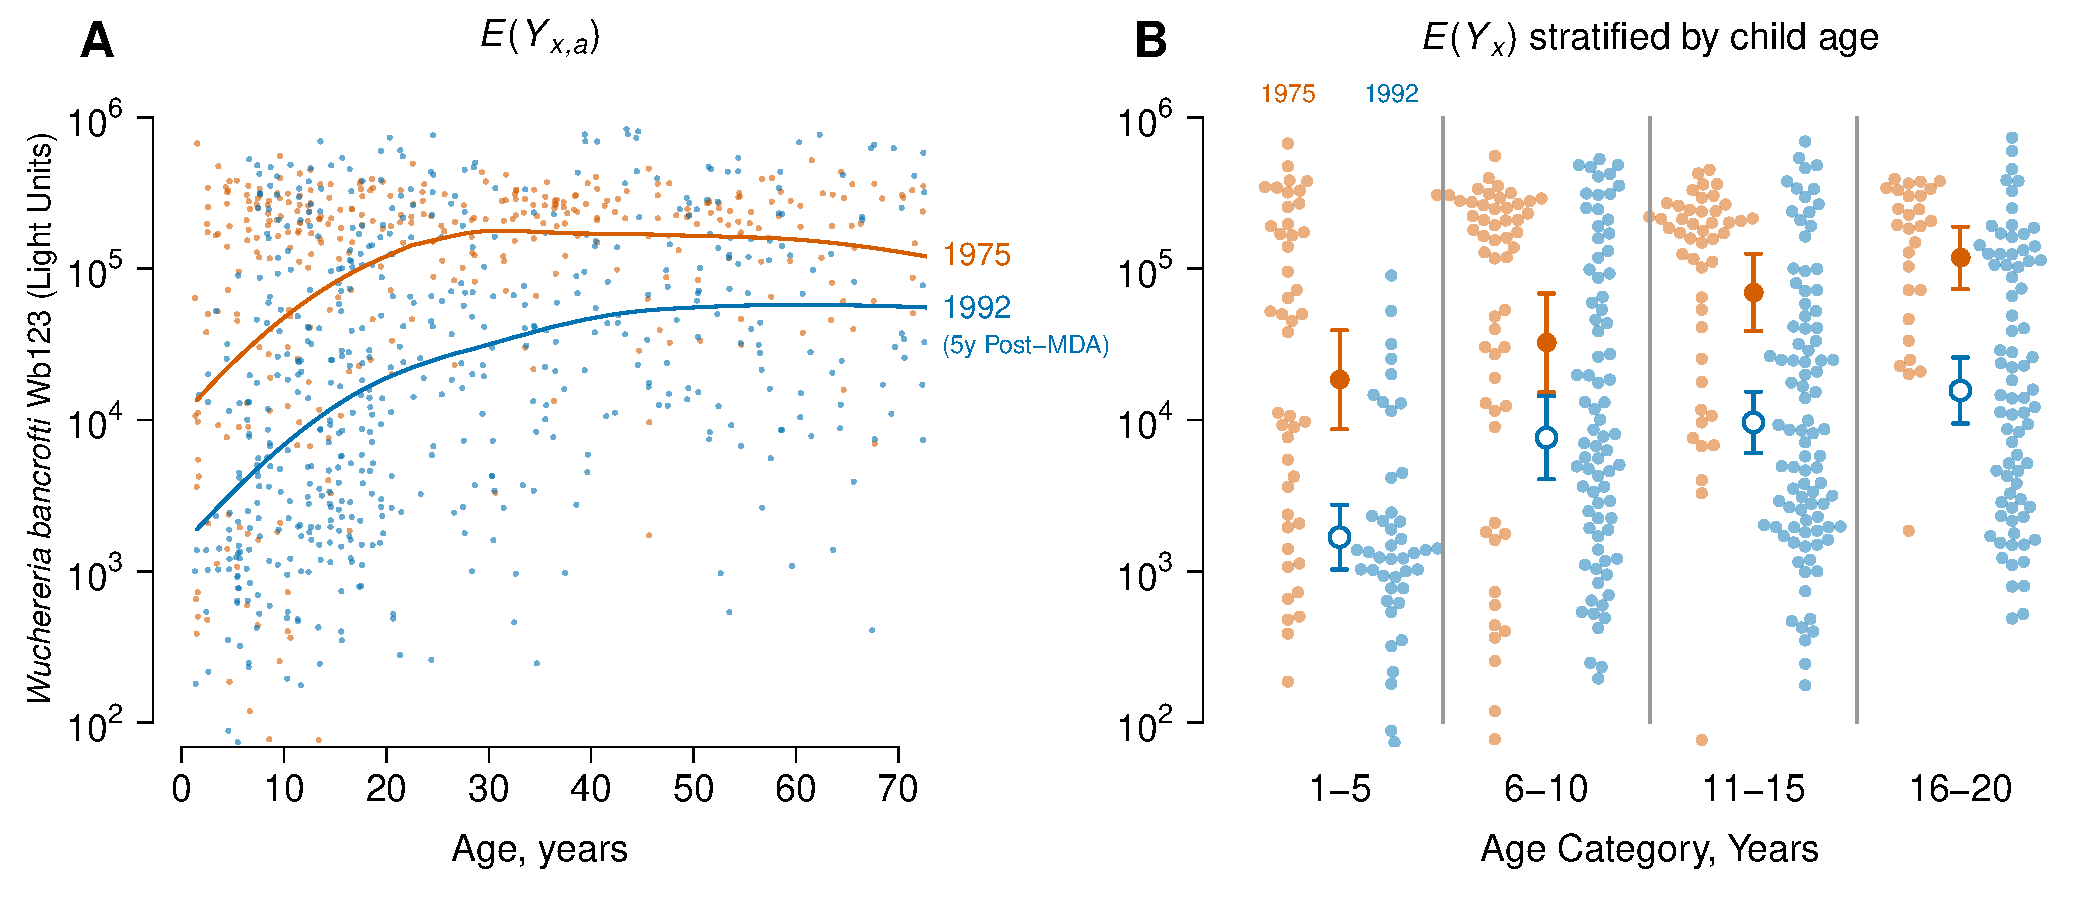
\includegraphics[width=\textwidth]{/users/benarnold/SLAbcurves/results/figs/mauke-Wb123-analysis.pdf}
\begin{minipage}{\textwidth}
\caption{Age-specific antibody response curves illustrating a shift in transmission intensity of \textit{Wuchereria bancrofti} due to mass drug administration (MDA) on Mauke Island.  Antibody response to the Wb123 antigen for \textit{W. bancrofti} measured in blood specimens with a luciferase immunoprecipitation system assay from residents in 1975 (N=362) before MDA and again in 1992 (N=553), five years following a single, island-wide MDA with diethylcarbamazine. \textbf{a}, The figure includes mean antibody levels $E(Y_{x,a})$ by survey year ($x$) and age ($a$) for ages 0-70 years; individual antibody responses (points) are shown along with summary curves fit with an ensemble machine learning algorithm (Online Methods). \textbf{b}, Age-adjusted geometric mean antibody response $E(Y_{x})$ and 95\% confidence intervals before (1975) and five years after (1992) MDA, stratified by 5 year age category (all differences significant at $P\leq0.01$ after Bonferroni correction).  }
\label{fig:mauke}
\end{minipage}
\end{center}
\end{figure}

%-------------------------------------------------------------------------------------------
% Figure 3 - Enterics
%-------------------------------------------------------------------------------------------

\begin{figure}[htbp]
\begin{center}
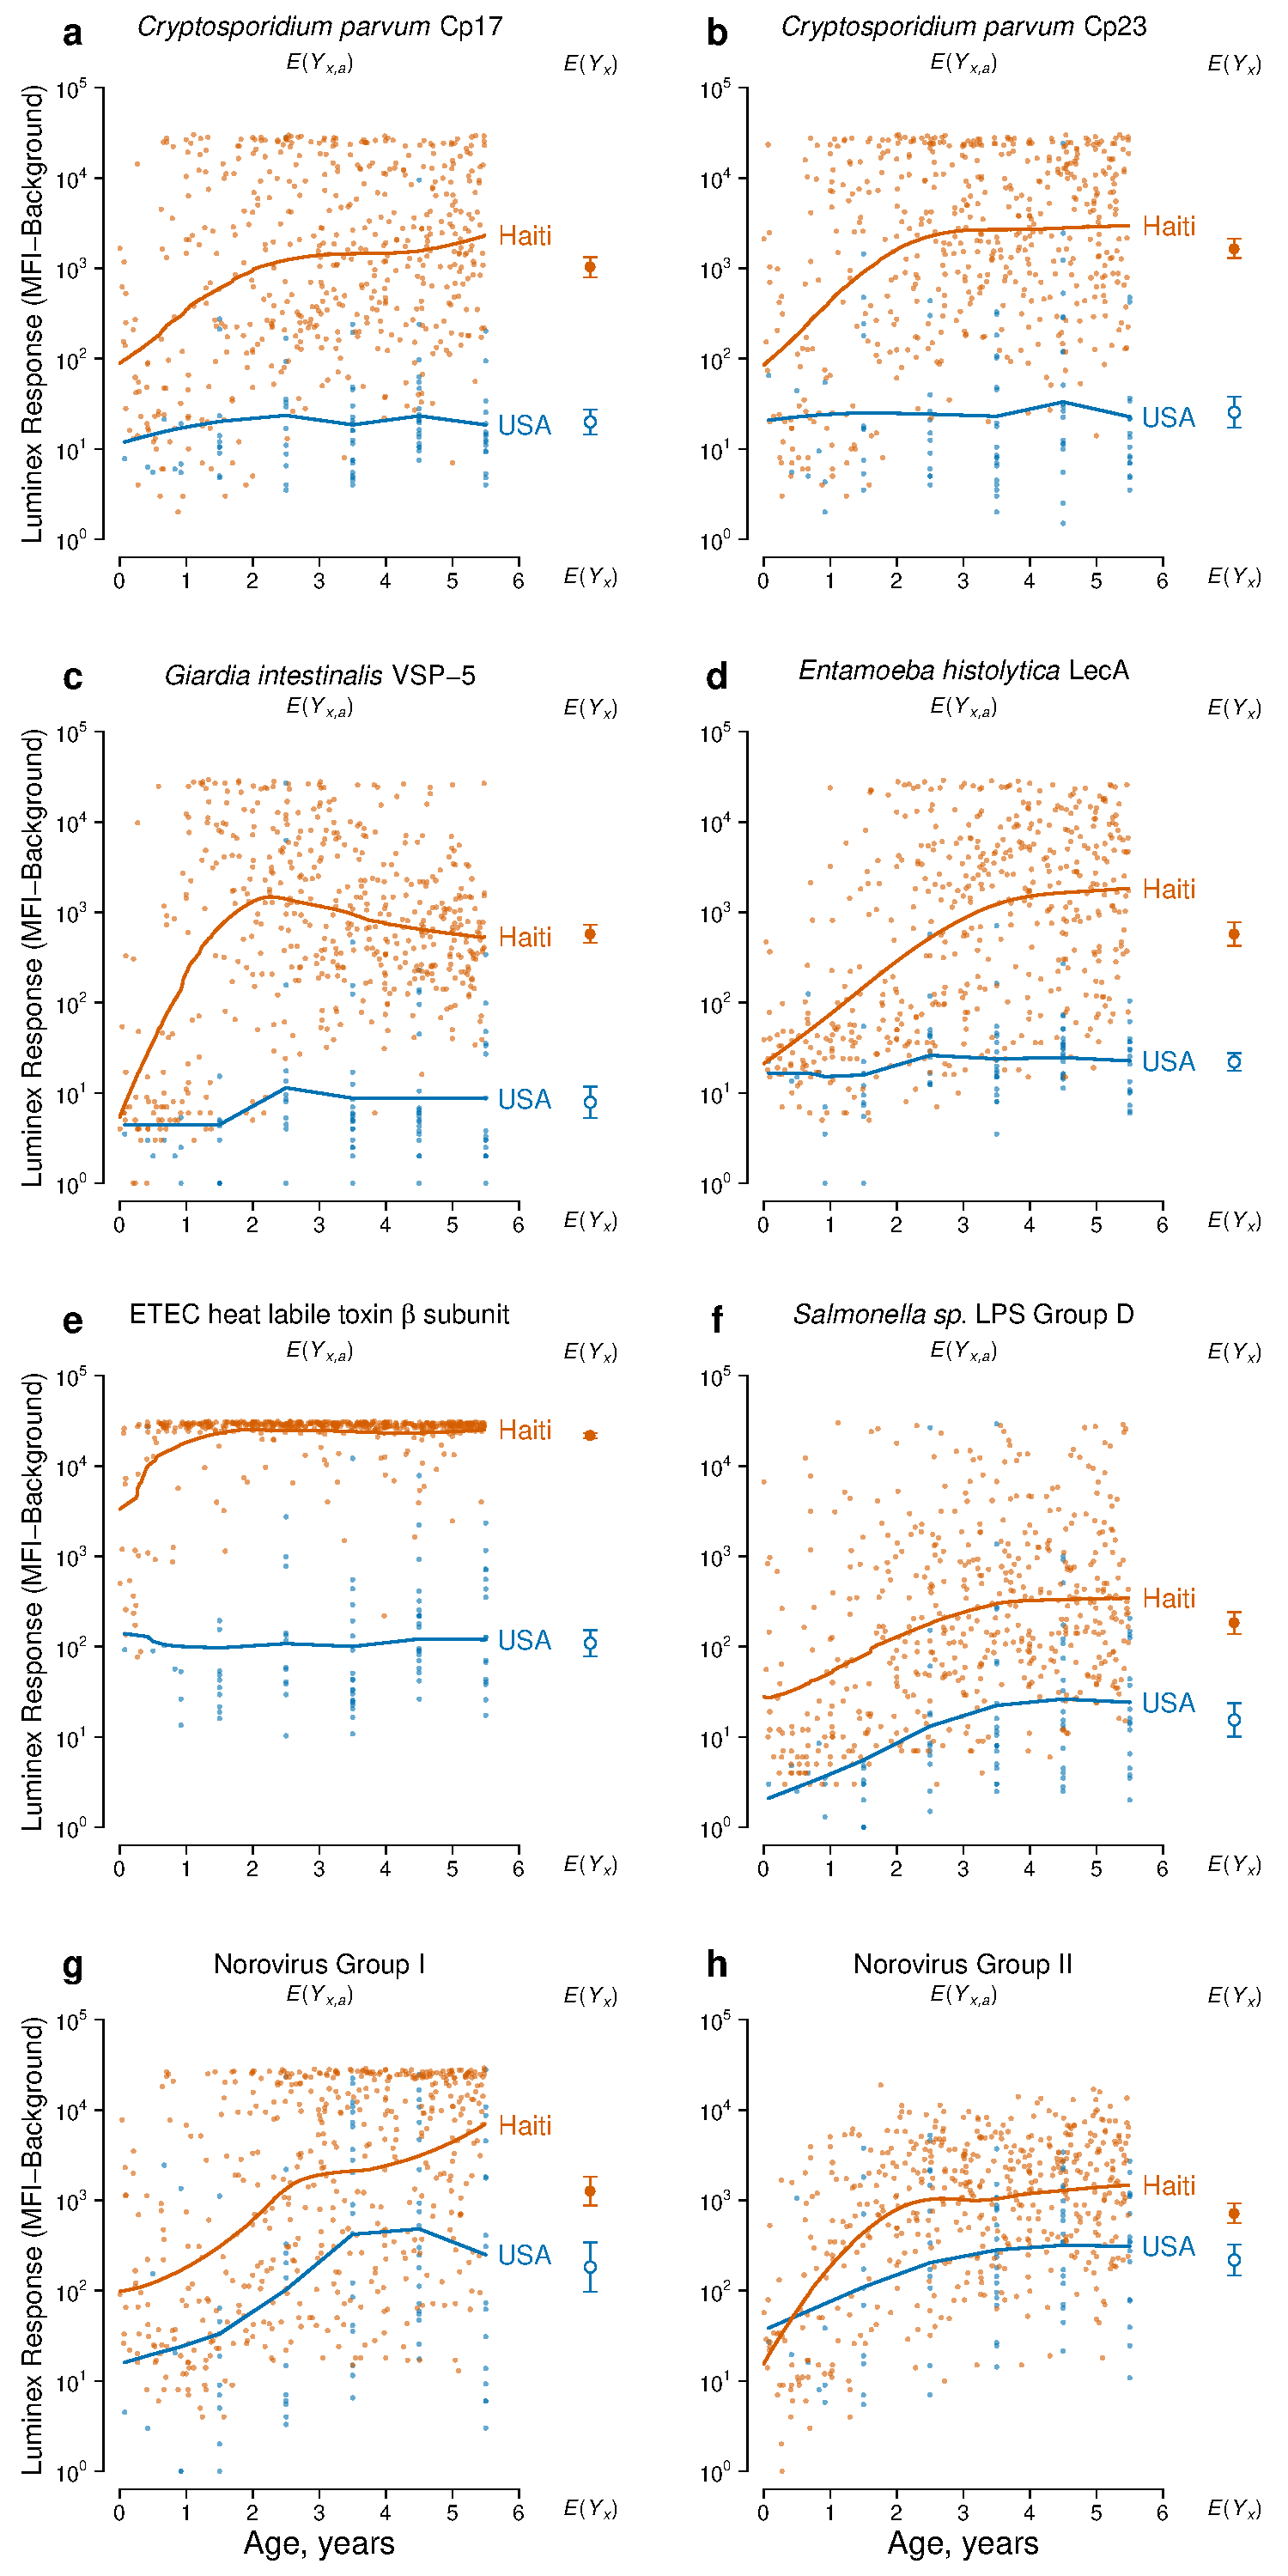
\includegraphics[width=0.7\textwidth]{/users/benarnold/SLAbcurves/results/figs/haiti2-USA-enterics-SL-curves.pdf}
\begin{minipage}{\textwidth}
\caption{caption on the next page}
\label{fig:enterics}
\end{minipage}
\end{center}
\end{figure}

\clearpage
Figure 3: Differences in enteric pathogen transmission between children in Leogane, Haiti (N=511) and the United States (USA) (N=86) measured by age-specific antibody response curves. Antibody response measured as median fluorescence intensity (MFI) minus background in multiplex bead assays on the Luminex platform. In each panel, individual antibody responses (points) are shown along with age-specific summary curves, $E(Y_{x,a})$, by country ($x$) and age ($a$), fit with an ensemble machine learning algorithm (Online Methods). Each panel also includes the geometric mean by country, $E(Y_{x})$, with error bars indicating 95\% confidence intervals (all differences significant at $P\leq0.01$ after Bonferroni correction).
\textbf{a.} \textit{Cryptosporidium parvum} recombinant 17-kDa antigen;
\textbf{b.} \textit{Cryptosporidium parvum} recombinant 27-kDa antigen;
\textbf{c.} \textit{Giardia intestinalis} variant-specific surface protein-5 (VSP-5);
\textbf{d.} \textit{Entamoeba histolytica} lectin adhesion molecule (LecA);
\textbf{e.} enterotoxigenic \textit{Escherichia coli} (ETEC) heat labile toxin $\beta$ subunit;
\textbf{f.} \textit{Salmonella sp.} lipopolysaccaride (LPS) Group D;
\textbf{g.} Norovirus Group I (xx additional details needed);
\textbf{h.} Norovirus Group II (xx additional details needed).

%-------------------------------------------------------------------------------------------
% Supporting information figures
%-------------------------------------------------------------------------------------------
\clearpage
\begin{center}
{\Large Extended Data Figures}
\end{center}
\vspace{50pt}

% set Table and Figure Numbering to have an "S" prefix
%\renewcommand{\thetable}{S\arabic{table}}
\setcounter{figure}{0} 
%\renewcommand{\thefigure}{S\arabic{figure}}



%-------------------------------------------------------------------------------------------
%  EIR results
%-------------------------------------------------------------------------------------------
%\clearpage
%\begin{figure}[htbp]
%\begin{center}
%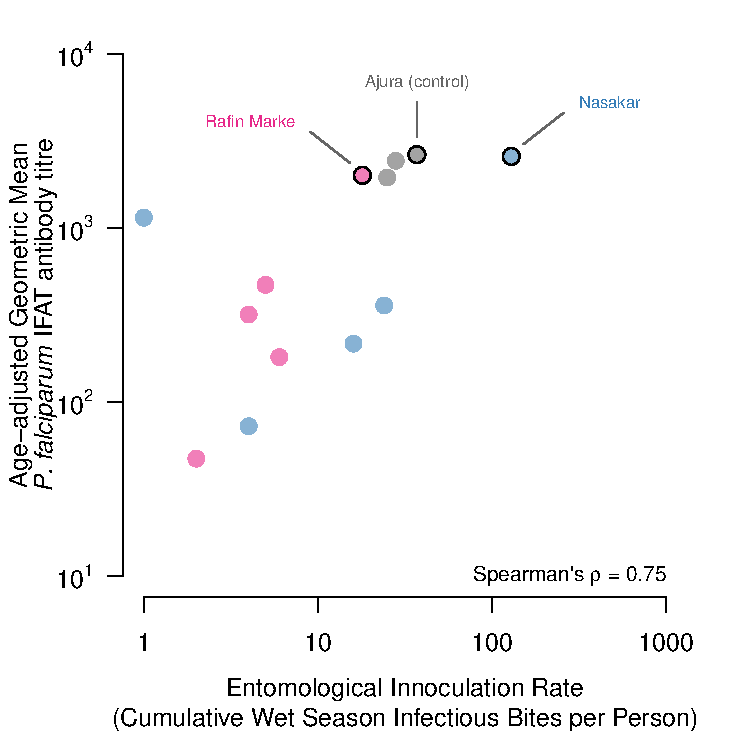
\includegraphics[width=0.75\textwidth]{/users/benarnold/SLAbcurves/results/figs/garki-IFATPf-EIR.pdf}
%\begin{minipage}{\textwidth}
%\caption{Village-level, age-adjusted geometric mean \textit{Plasmodium falciparum} indirect fluorescent antibody (IFA) test titres, $E(Y_x)$, versus wet season entomological innoculation rate (EIR) in the three study villages with both entomological and serological measurements in the Garki project, Nigeria. Ajura was a control village (no treatment) while Rafine Marke and Nasakar received a combination of insecticide spraying and mass drug administration of surfanene-pyrimethamine in 1972-1973. The intervention villages also received targeted distribution of chloroquine to children <10 and self-reporting fever cases in the 1974-75 post-intervention period. The circled and labeled points are from the 1971 wet season (pre-intervention) and other points represent wet seasons for 1972-73 (Ajura) or 1972-75 (Rafine Marke and Nasakar).  The EIR estimates were previously published in Table 4 of Molineaux et al. 1980. The EIR represents the number of sporozoite positive bites per person over each wet season, and was estimated by multiplying the man-biting rate by the sporozoite positive rate in night-bite collections. Night-bite collections were conducted every 2 weeks using 2 indoor and 2 outdoor stations per village, with 2 human bait collectors in each station throughout the night. A single data point outside the figure range is not shown (Nasakar 1972, EIR value = 0, $E(Y_x) = 10^{3.0591}$), but was included in the Spearman rank correlation estimate.  }
%\label{fig:garkiEIR}
%\end{minipage}
%\end{center}
%\end{figure}

%-------------------------------------------------------------------------------------------
% Figure S1 - Garki village level results
%-------------------------------------------------------------------------------------------
\clearpage
\begin{figure}[htbp]
\begin{center}
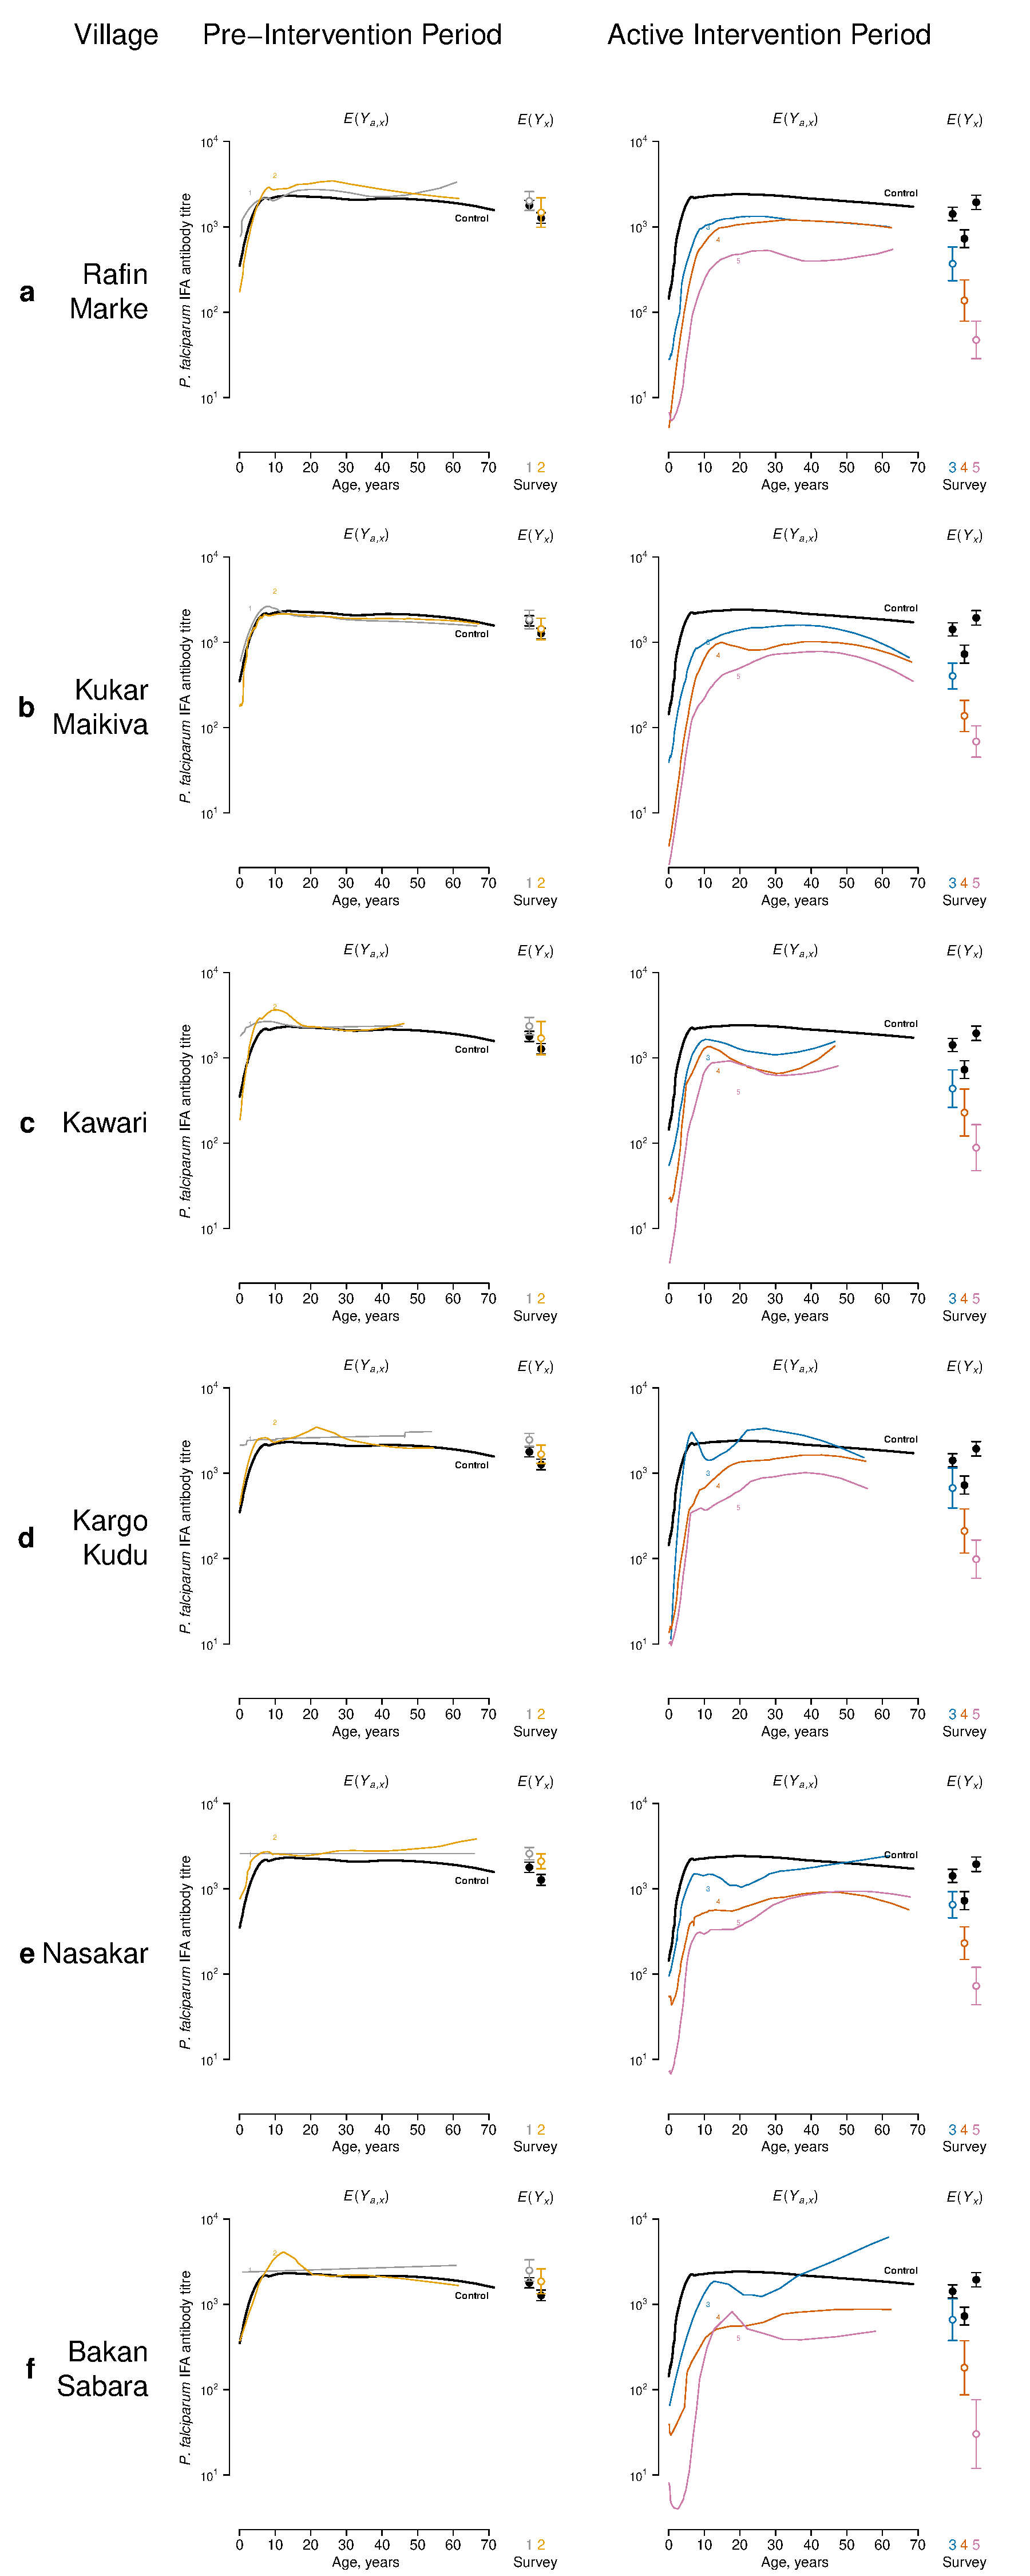
\includegraphics[width=0.6\textwidth]{/users/benarnold/SLAbcurves/results/figs/garki-IFAPf-by-village.pdf}
\begin{minipage}{\textwidth}
\caption{Caption on the following page.}
\label{fig:garkiVillageEy}
\end{minipage}
\end{center}
\end{figure}
\clearpage
Figure 1: Age-specific antibody curves estimated separately for each intervention village (\textbf{a-f}) measure changes in malaria transmission due to intervention in the Garki Project, Nigeria (1970-1976).  Antibody response measured with the indirect fluorescent antibody (IFA) test for \textit{Plasmodium falciparum}. Pre-intervention period wet and dry seasons measures (survey rounds 1-2) and active intervention period (survey rounds 3-5, at 20, 50, and 70 weeks following the start of intervention) are plotted.  Age-specific antibody curves, $E(Y_{x,a})$ by group ($x$) and age ($a$), were estimated nonparametrically from quantitative antibody responses in individuals using an ensemble machine learning algorithm (Online Methods). Control measurements were combined across survey rounds within each period when plotting the curves to facilitate visual comparison of shifts in transmission intensity between surveys. Age-adjusted geometric means by group, $E(Y_x)$, provide summary differences between curves at each survey round. Error bars show 95\% confidence intervals for the age-adjusted geometric means.


%-------------------------------------------------------------------------------------------
% Figure S2 - Miton E(Yx,a) and E(Yx) estimates
%-------------------------------------------------------------------------------------------
\clearpage
\begin{figure}[htbp]
\begin{center}
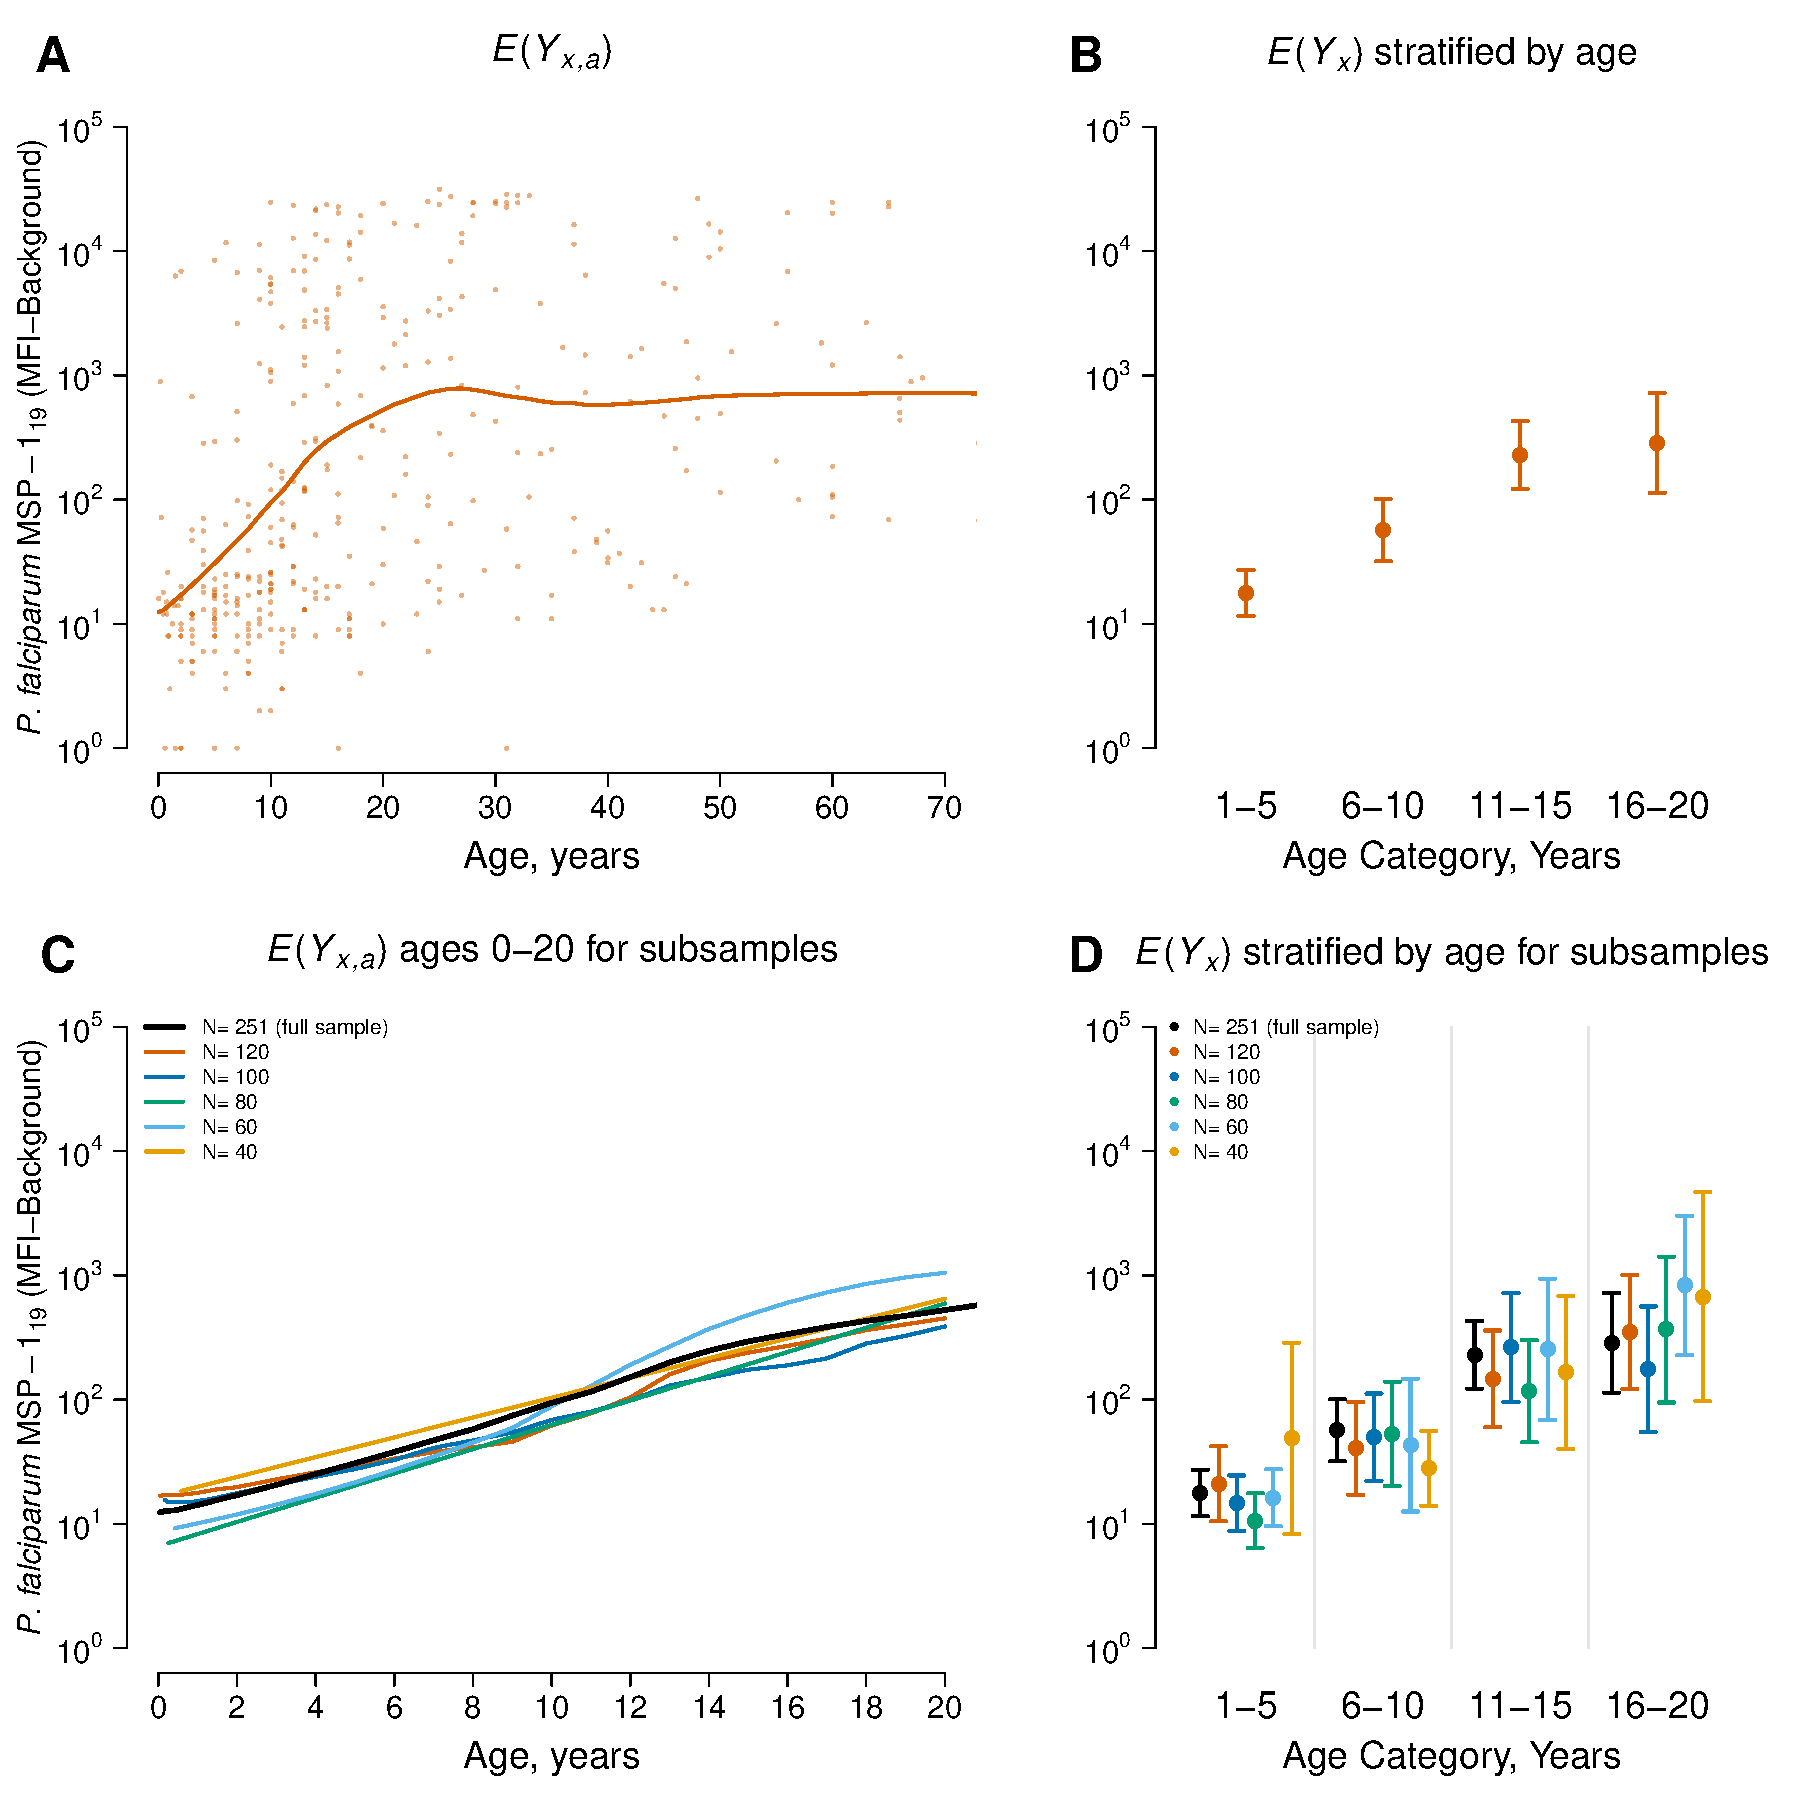
\includegraphics[width=\textwidth]{/users/benarnold/SLAbcurves/results/figs/miton-msp1-analysis.pdf}
\begin{minipage}{\textwidth}
\caption{Age-specific antibody response curve for immunoglobulin G antibody response to the \textit{Plasmodium falciparum} merozoite surface protein-$1_{19}$ (MSP-$1_{19}$) antigen in a 1998 cross-sectional measurement of 383 individuals in the community of Miton, Haiti (xxcitexx). A recombinant GST/MSP-$1_{19}$ fusion protein cloned from the \textit{P. falciparum} isolate 3D7 was included in a multiplex bead assay on the Luminex platform. (\textbf{a}) Mean antibody levels $E(Y_{x,a})$ by age ($a$) for ages 0-70 years; individual antibody responses (points) are shown along with a summary curve fit with an ensemble machine learning algorithm (Online Methods). (\textbf{b}) Age-adjusted geometric mean antibody response $E(Y_{x})$ and 95\% confidence intervals stratified by 5 year age category estimated using targeted minimum loss-based estimation (Online Methods). The number of individuals in each age group was: 1-5 (N=69), 6-10 (N=74), 11-15 (N=68), and 16-20 (N=40). In this example there is no stratification by group ($x$), but we have left the notation unchanged from other examples to make clear the comparison with other examples in the paper, such as Fig 1.}
\label{fig:mitonEYxa}
\end{minipage}
\end{center}
\end{figure}

%-------------------------------------------------------------------------------------------
% Figure S3 - Mauke results
%-------------------------------------------------------------------------------------------
\begin{figure}[htbp]
\begin{center}
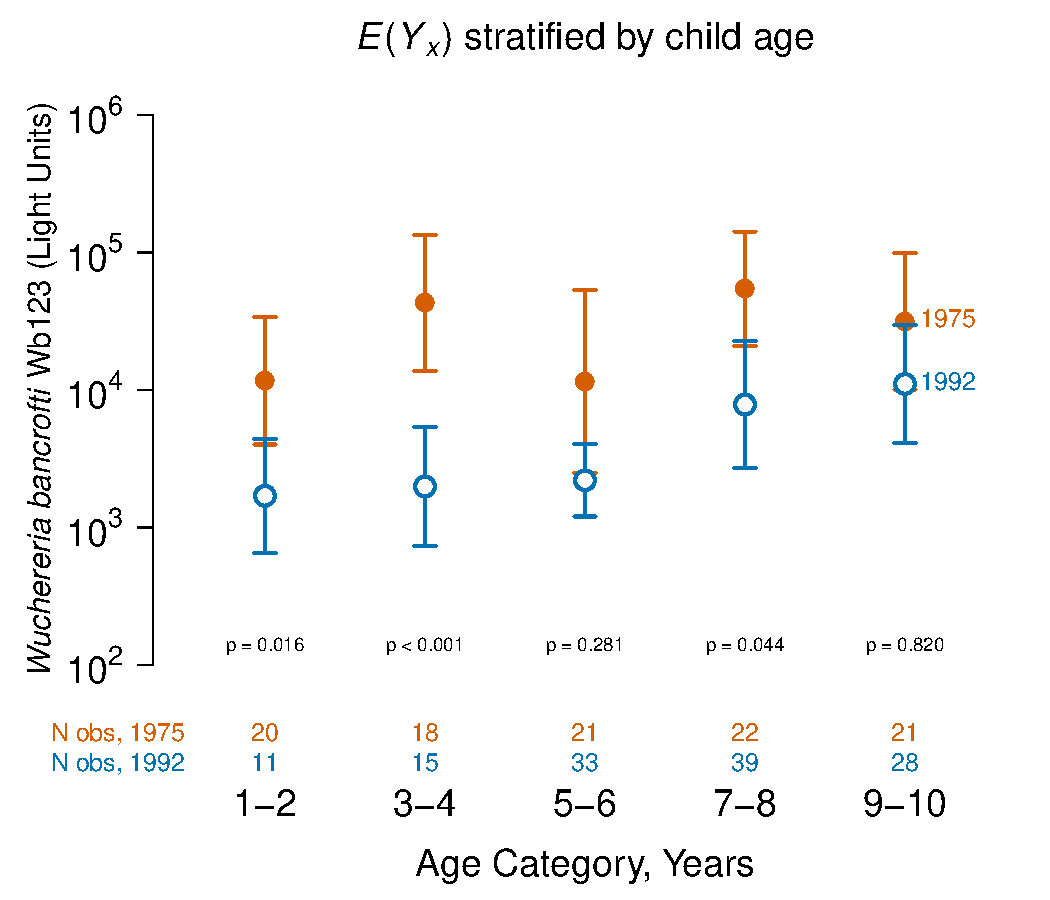
\includegraphics[width=0.75\textwidth]{/users/benarnold/SLAbcurves/results/figs/mauke-Wb123-analysis-2y.pdf}
\begin{minipage}{0.75\textwidth}
\caption{Age-adjusted geometric mean antibody response $E(Y_{x})$ and 95\% confidence intervals to the Wb123 antigen for \textit{WWuchereria bancrofti} in 1975 and in 1992. The 1992 survey was five years after a single, island-wide mass drug administration (MDA) with diethylcarbamazine. The means are stratified by 2 year age band. The number of observations per stratum (N obs) is listed and $P$-values are Bonferroni-corrected tests of differences between means in each stratum.}
\label{fig:maukeS4}
\end{minipage}
\end{center}
\end{figure}

%-------------------------------------------------------------------------------------------
% Figure S4 - Logan results
%-------------------------------------------------------------------------------------------
\clearpage
\begin{figure}[htbp]
\begin{center}
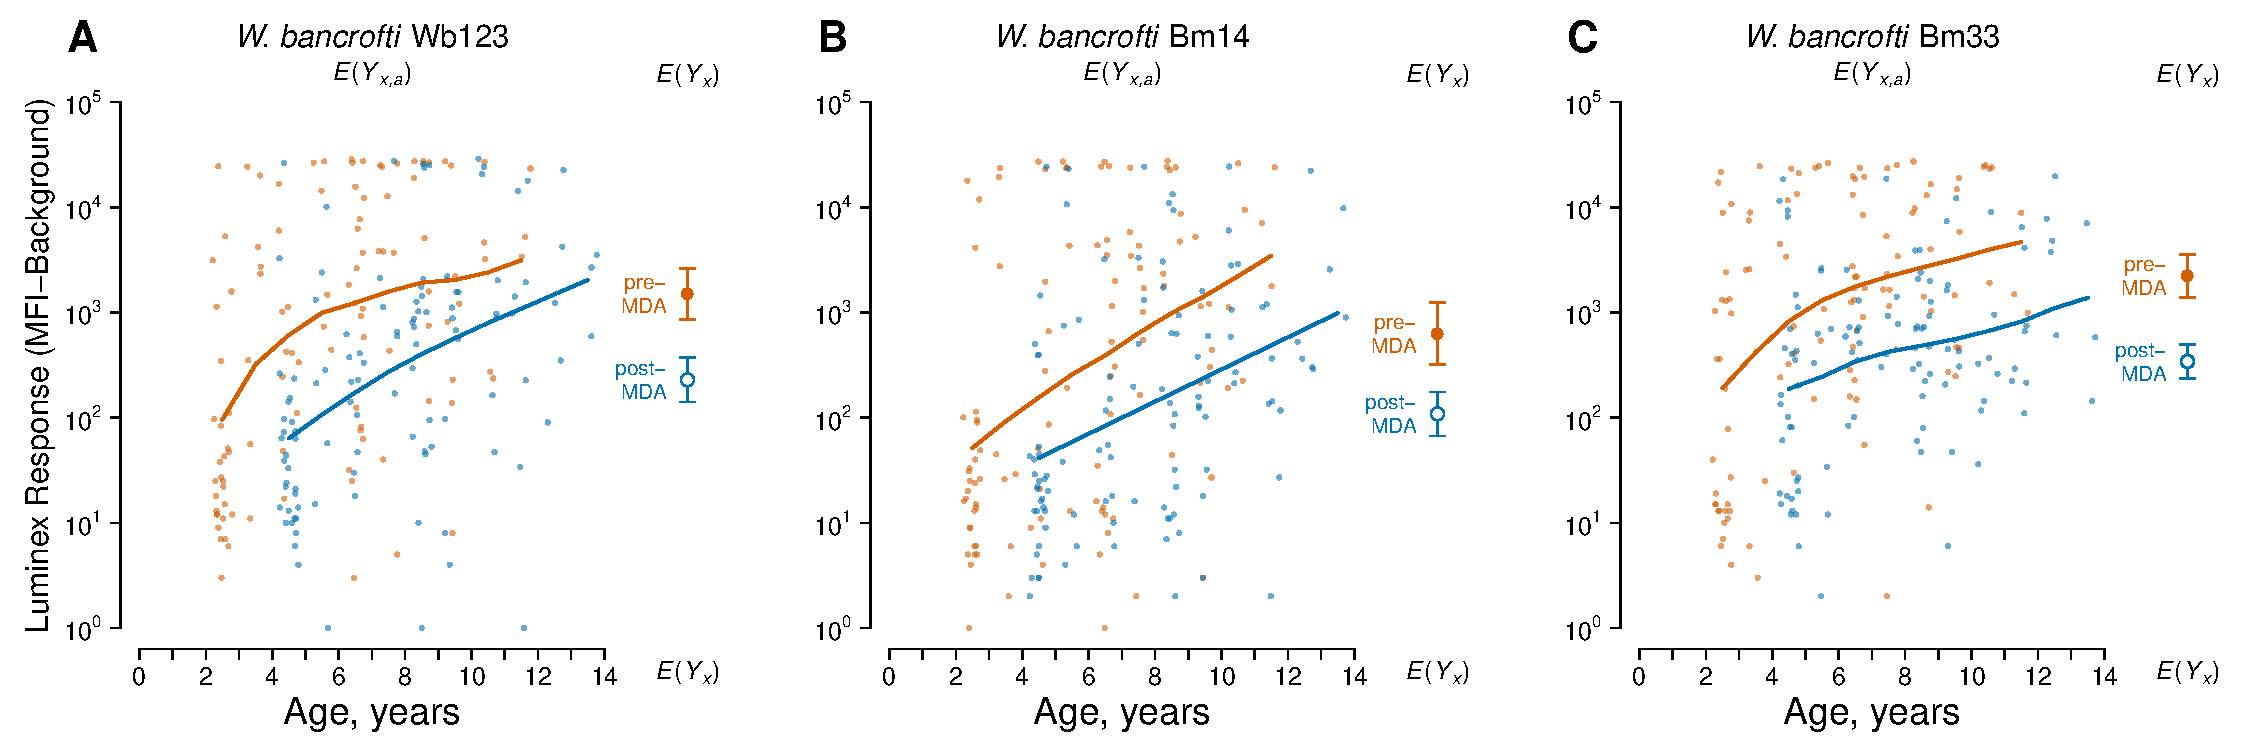
\includegraphics[width=\textwidth]{/users/benarnold/SLAbcurves/results/figs/caira-LF-curves.pdf}
\begin{minipage}{\textwidth}
\caption{Age-specific antibody response curves, $E(Y_{x,a})$ illustrating a shift in transmission intensity of \textit{Wuchereria bancrofti} due to mass drug administration (MDA) with diethylcarbamazine and albendazole in an encampment of internally displaced people, Leogane, Haiti 2011-2013.  IgG antibody response measured as median fluorescence intensity (MFI) minus background in multiplex bead assays on the Luminex platform for Wb123 (\textbf{a}), Bm14 (\textbf{b}), and Bm33 (\textbf{c}) antigens. Individual antibody responses (points) are shown along with summary curves fit with an ensemble machine learning algorithm (Online Methods). Blood specimens were collected from 110 children ages 2-11 at enrollment in two rounds: the pre-MDA measurement was conducted in November 2011, and the post-MDA measurement was conducted in November 2013.  MDA campaigns took place in January 2012 and January 2013. Age-adjusted geometric mean estimates, $E(Y_x)$ were estimated only using measurements in areas of overlap between the curves from ages 4 though 11 years old (N=73 in pre-MDA and N=102 in post-MDA measurements). All differences significant at $P<0.0001$.}
\label{fig:cairaS5}
\end{minipage}
\end{center}
\end{figure}

%-------------------------------------------------------------------------------------------
% Figure S5 - Mauke seroprevalence curves
%-------------------------------------------------------------------------------------------
\clearpage
\begin{figure}[htbp]
\begin{center}
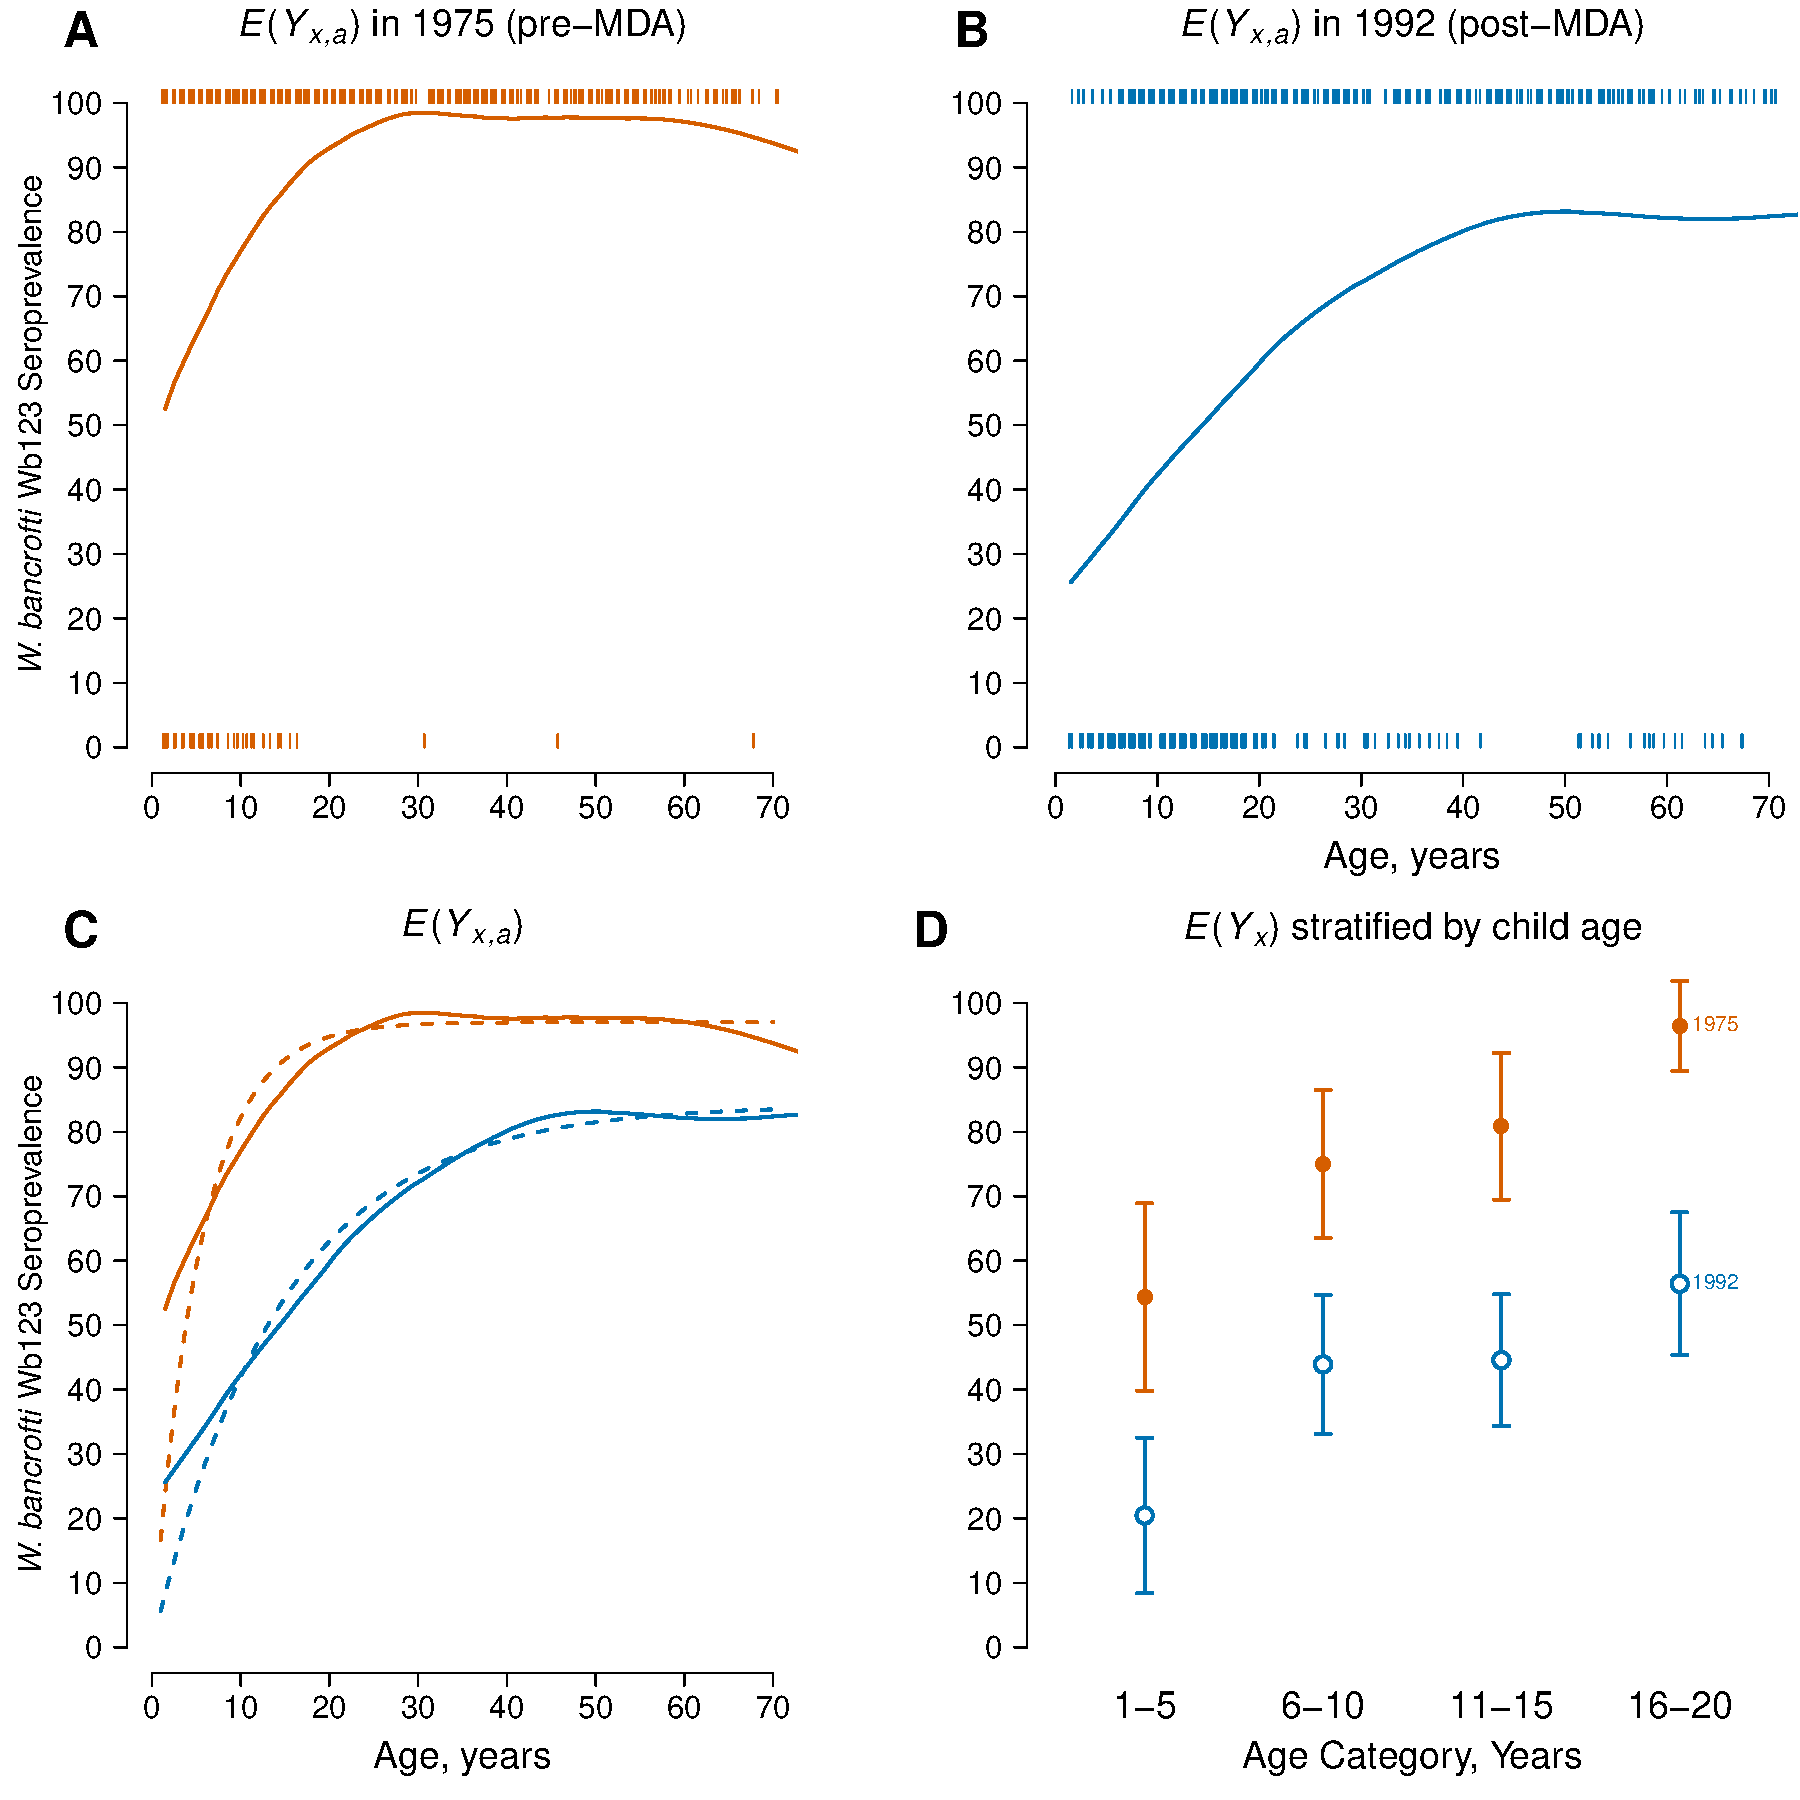
\includegraphics[width=\textwidth]{/users/benarnold/SLAbcurves/results/figs/mauke-Wb123-binary.pdf}
\begin{minipage}{\textwidth}
\caption{Illustration of the methodology applied to binary (seropositive / seronegative) antibody measurements, typical of rapid diagnostic test results. Age-specific antibody response curves illustrating a shift in transmission intensity of \textit{Wuchereria bancrofti} due to mass drug administration (MDA) on Mauke Island.  Antibody response to the Wb123 antigen for \textit{W. bancrofti} measured in blood specimens with a luciferase immunoprecipitation system assay from residents in 1975 (N=362) before MDA and again in 1992 (N=553), five years following a single, island-wide MDA with diethylcarbamazine. The quantitative antibody levels were reduced to seropositive and seronegative status using a previously determined cutoff value of 10968 with sensitivity >98\% and specificity >84\%.$^{37}$ Age-specific seroprevalence curves $E(Y_{x,a})$ in 1975 (\textbf{a}) and 1992 (\textbf{b}); rug plots include individual data points and summary curves were fit with an ensemble machine learning algorithm (Online Methods). \textbf{c}, overlay of the curves in the two survey years to illustrate the shift due to lower transmission.  \textbf{d}, age-adjusted seroprevalence $E(Y_{x})$ and 95\% confidence intervals before (1975) and five years after (1992) MDA, stratified by 5 year age category (all differences significant at $P\leq0.01$ after Bonferroni correction).}
\label{fig:maukebina}
\end{minipage}
\end{center}
\end{figure}





\end{document}